\documentclass[12pt]{article}

\usepackage{amsmath}
\usepackage{amsfonts}
\usepackage{amssymb}
\usepackage{graphicx}
\usepackage[center]{caption}
\usepackage{mathtools}
\usepackage{lipsum}
\usepackage{stackengine}
\usepackage{fancyhdr}
\usepackage{caption}
\usepackage{tikz}
\usetikzlibrary{shapes.geometric, arrows}
\usepackage{float}
\usepackage[a4paper,left=1in,right=1in,top=1in,bottom=1in,footskip=.25in]{geometry}
\usepackage{etoolbox}
\usepackage[nottoc]{tocbibind}
\usepackage{tabu}
\usepackage{enumitem,kantlipsum}
\usepackage{verbatim}
\usepackage{hyperref}
\begin{document}


\section{Aim}
This test case is for checking the capability of the written Isogeometric analysis code with an Electrical loading.
\section{Problem description}\label{2DPWPELPD}
\emph{Section 7.2.1 in Documentation}\\
A 2D plate is subjected to Electrical loading as shown in Figure(\ref{PureElectrical22}).The material used is PZT-PIC151 ceramics.\\
The movement of bottom edge AB is fixed in y-direction and left edge AC in x-direction.The top edge CD is grounded ( potential = 0 volts). An electrical potential V of 100 volts is applied on bottom edge AB as shown in Fig. (\ref{PureElectrical22})
\begin{figure}[H]
	\centering
	\begin{minipage}{.4\textwidth}
		\centering
		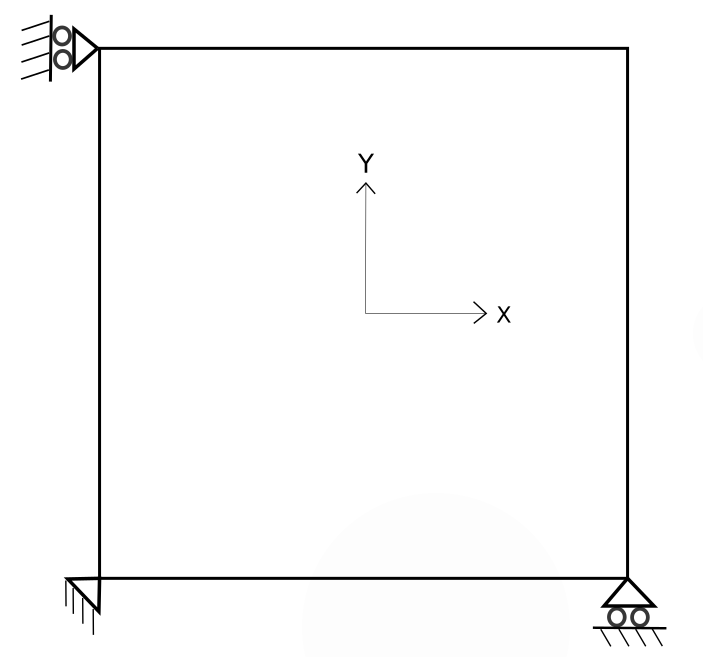
\includegraphics[width=0.8\linewidth]{2DPlate.png}
		\captionof{figure}{2D Plate}
		\label{2Dplate}
	\end{minipage}%
	\begin{minipage}{.4\textwidth}
		\centering
		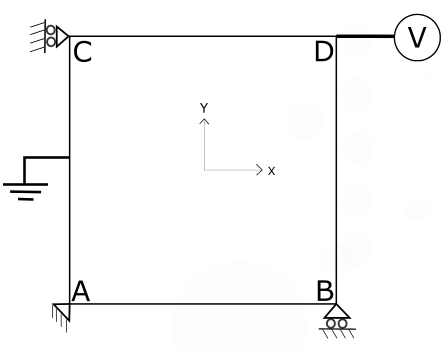
\includegraphics[width=1\linewidth]{PureElectrical.png}
		\captionof{figure}{2D Plate with pure electrical loading}
		\label{PureElectrical22}
	\end{minipage}
\end{figure}

\newpage

\section{How to run the Program}
\begin{enumerate}[leftmargin=*]
	\item The code is written in python and external libraries numpy, matplotlib.pyplot, sys, path from pathlib and math are used.
	\item Please use any environment which will compile python programs
	\item Place all the files in a single folder.
	\item A file named Input.py can be edited to change the dimensions of the plate. User can change Length, Height and Thickness of the plate. \\(The results discussed below are for Length = 10 mm, Height = 10 mm and Thickness = 1 mm)
	\begin{figure}[H]
		\begin{center}
			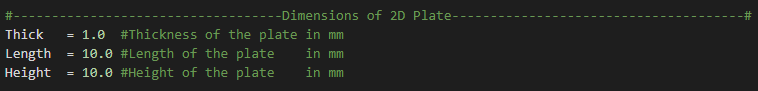
\includegraphics[scale=0.8]{Input.png} 
		\end{center}	
	\end{figure}
	\item Before you run the file, please make sure that the working directory is same as the folder  which
	Consists the Program.
	\item Use command  $>>>$ python Main\_Program.py to run the program.
	\item The contour plots will be saved in the folder \textbf{Results.}
	\item A "log.txt" file is created in the same folder which contains the values of the results plotted.
	
	
\end{enumerate}

\newpage

\section{Results and discussions}
In this section the comparison is made between IGA code generated result and Abaqus plane strain full integration piezoelectric element (\textbf{CPE4E}).\\The below figures shows the values of Electrical potentials (EPOT) and reactive electrical nodal charge (RCHG) for both Abaqus and IGA element.\\
\\\textbf{Electro-mechanical coupling is deactivated in this case by giving all the piezoelectric constants a value of "zero"  }
\\
\textbf{A similar contour is used for the program generated results and the Abaqus results for easy comparison. }\\
\\
Figure(\ref{E1EPOT}) and Figure(\ref{E1EPOT_IGA}) show the Electrical potential (EPOT) values of the single CPE4E element and single IGA element at 100 \% loading respectively. \\
\begin{figure}[H]
	\centering
	\begin{minipage}{.5\textwidth}
		\centering
		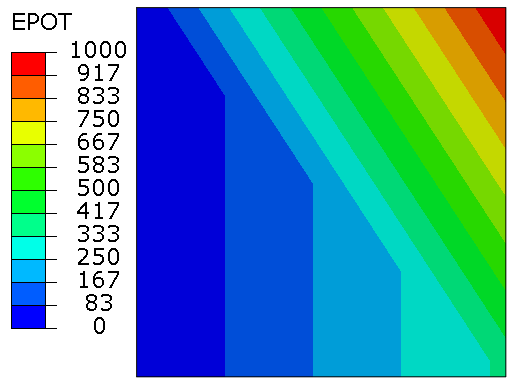
\includegraphics[width=1\linewidth]{E1EPOT.png}
		\captionof{figure}{CPE4E Element:EPOT \\\textbf{Abaqus generated result}}
		\label{E1EPOT}
	\end{minipage}%
	\begin{minipage}{.7\textwidth}
		\centering
		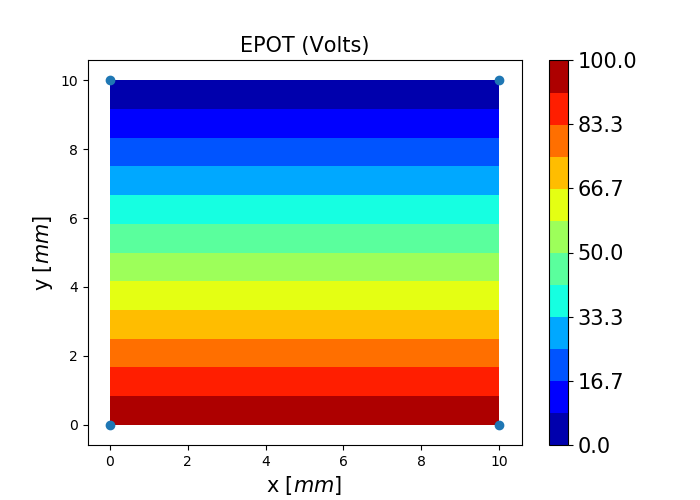
\includegraphics[width=1\linewidth]{E1EPOT_IGA.png}
		\captionof{figure}{IGA Element:EPOT \\ \textbf{Program generated result}}
		\label{E1EPOT_IGA}
	\end{minipage}
\end{figure}
\begin{comment}
\begin{figure}[H]
\begin{center}
\includegraphics[scale=0.45]{xyz.png} 
\caption{\\CPE4 Element U1}\label{xyz}
\end{center}	
\end{figure}

\begin{figure}[H]
\begin{center}
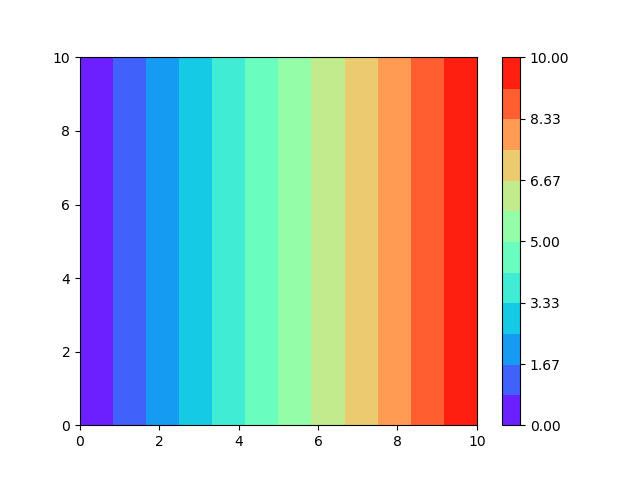
\includegraphics[scale=0.8]{Figure_1.png} 
\caption{\\IGA Element U1}\label{Figure_1}
\end{center}	
\end{figure}
\end{comment}
Figure(\ref{E1RCHG}) and Figure(\ref{E1RCHG_IGA}) show the reactive nodal charge (RCHG) values of the single CPE4E element and single IGA element at 100 \% loading respectively. \\
\begin{figure}[H]
	\centering
	\begin{minipage}{.5\textwidth}
		\centering
		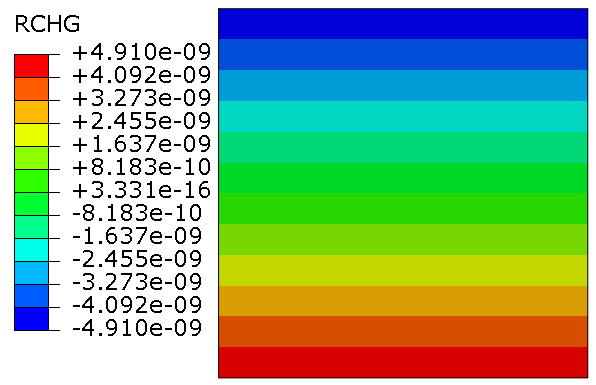
\includegraphics[width=1\linewidth]{E1RCHG.png}
		\captionof{figure}{CPE4 Element:RCHG
			\\\textbf{Abaqus generated result}}
		\label{E1RCHG}
	\end{minipage}%
	\begin{minipage}{.6\textwidth}
		\centering
		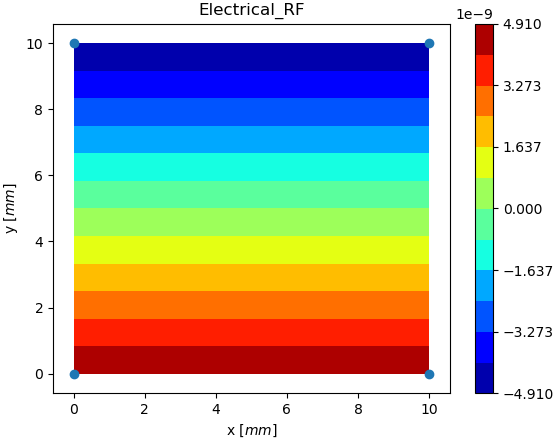
\includegraphics[width=1\linewidth]{E1RCHG_IGA.png}
		\captionof{figure}{IGA Element:RCHG \\ \textbf{Program generated result}}
		\label{E1RCHG_IGA}
	\end{minipage}
\end{figure}


\end{document}